\section{Common terminologies}

This section defines common terminologies that are used throughout the paper.

\subsection{Pipeline}

Our goal is to associate each bit with a resolution level and a bit plane. To introduce the concept
of resolution to gridded data, we use the discrete wavelet transform, in particular, the popular
CDF5/3 [CITE] transform. For precision, we quantize the floating-point wavelet coefficients to
$16$-bit signed integers, thereby eliminating the exponent bits so that every bit can be associated
with a bit plane. To further avoid special treatment of the sign bit in two's complement form, we
convert the quantized coefficients to negabinary form [CITE]. This transformation increase the
number of bit planes from $16$ to $17$.

In practice, bits are never read and transmitted one by one, so in this paper, our fundamental unit
of data is a \emph{chunk} of bits. A \emph{chunks} is a bit plane of a group of $4\times 4$
coefficients in the same subband (the multi-dimensional wavelet transform rearranges the
coefficients into subbands [CITE], each can be thought of as a resolution level). Each group hence
contains $17$ chunks. For all the experiments in this paper, we perform the wavelet transform $3$
times in each dimension, producing $10$ subbands in 2D and $22$ subbands in 3D. Figure
\ref{fig:pipeline} illustrates how all these steps fit together to produce a stream of chunks from
the original, raw data.

\begin{figure}
  \centering
  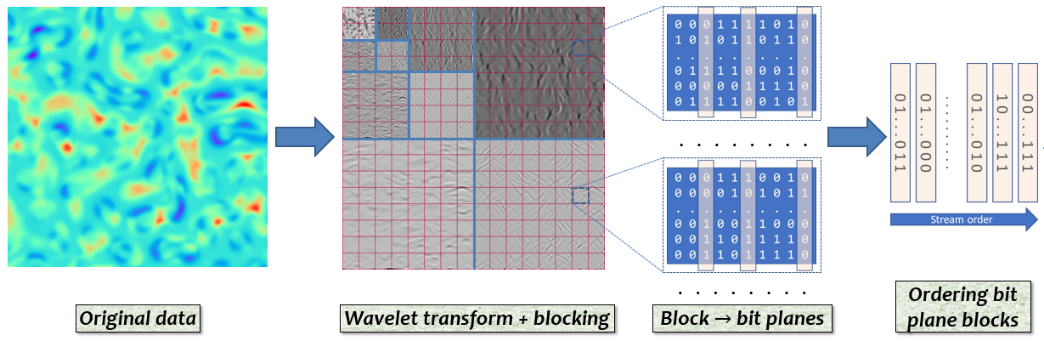
\includegraphics[width=\linewidth]{img/pipeline.png}
  \caption{Our data stream creation pipeline. The input is a regular grid, the output is a stream of
  chunks, where each chunk is a bit plane from a group of quantized wavelet coefficients stored in
  negabinary format. The subbands are separated by blue lines in the second image, with the coarsest
  subband at the top left corner. TODO: revise this figure}
  \label{fig:pipeline}
\end{figure}

\subsection{Stream signature}

To analyze the core characteristics of a stream, we introduce the concept of a stream
\emph{signature}. A signature is a $B \times L$ matrix, with $B$ being the number of bit planes, and
$S$ being the number of subbands produced by the wavelet transform. A chunk on subband $s$ and bit
plane $b$ can be associated with the $b, l$ cell of the matrix. Every chunk in the stream can be
associated with one (and only one) of the cells. Each matrix cell $(b,l)$ contains a value in the
range of $[0,B\times L)$, indicating the position in which chunks of that cell appear in the stream,
relative to chunks of all other cells, on average. It is our hypothesis that streams optimized for
different analysis tasks produce qualitatively distinctive signatures, and therefore, a set of
signatures can be pre-computed once and later picked to use depending on the analysis at hand.

To compute a stream signature, we partition the whole domain into several regions, compute one
chunks in each per-region signature are spatially related. The reason for this partitioning is that
it is only meaningful to study the relative ordering of cells if the chunks associated with those
cells all come from same region of the original domain. Ideally the global signature for a stream
should contain all the per-region signatures, but due to space constraint, as well as for ease of
visualization, we condense all the local signatures by averaging them on a per-cell basis, and only
study the average signature. (TODO: add the algorithm).

% \begin{algorithm}
%   \KwData{this text}
%   \KwResult{how to write algorithm with \LaTeX2e }
%   initialization\;
%   \While{not at end of this document}{
%    read current\;
%    \eIf{understand}{
%     go to next section\;
%     current section becomes this one\;
%     }{
%     go back to the beginning of current section\;
%    }
%   }
%   \caption{How to write algorithms}
% \end{algorithm}
